\entry{2026-10-14}{Second-order references (E0, complete): 3D pass, 2D pass with flags}

Lane \texttt{2026-10-06-jcp-references}, last commit \texttt{cc04f4b54}, mirror \texttt{66ee55015}. Cluster namespace \texttt{jcp-ref}; 39.7 GPU-h (A100 and H200). Every step was Codex-gated, and the final report audit is READY. Report: \path{worktrees/2026-10-06-jcp-references/experiments/jcp-references/report.md}. Loader: \texttt{refstore.py}. Numbers below are quoted from the lane's generated report.

\subsection*{Findings}
\begin{itemize}
\item \textbf{3D passes.} All 200 historical case-kinds pass the order check, with observed order 1.99--2.02. The median $\epsilon_{ref}$ is $\approx 2.5\times10^{-5}$ and the worst is $1.16\times10^{-4}$. The pseudo-spectral cross-check passes 8/8, with the measured distance equal to 1.00--1.02 of $\epsilon_{ref}$. Sealed cohort 128/128, OOD 32/32.
\item \textbf{2D passes with flags.} 191/204 historical case-kinds pass, with $\epsilon_{ref}\approx 3$--$4\times10^{-6}$ (space+time) and $\approx1.2\times10^{-7}$ (space only). The 13 flagged cases are not rankable:
  \begin{itemize}
  \item 12 high-viscosity space-only cases fail the (conservative) solver-floor check;
  \item test64 case 36 fails the order check.
  \end{itemize}
  The cross-check passes 8/8. Sealed cohort 230/256 accepted, OOD 64/64.
\item \textbf{How wrong the old first-order references were} (maximum over output times):
  \begin{itemize}
  \item 3D: median 0.7\,\%, maximum 2.81\,\%;
  \item 2D: median 0.03--0.08\,\%, maximum 0.35\,\%.
  \end{itemize}
  So 3D numbers can move noticeably on re-scoring, and 2D numbers barely.
\item \textbf{Controls fired.} A deliberately first-order solver and an injected first-order defect are both rejected. The cross-check against the old references fails on 16/16 cases.
\end{itemize}
\begin{center}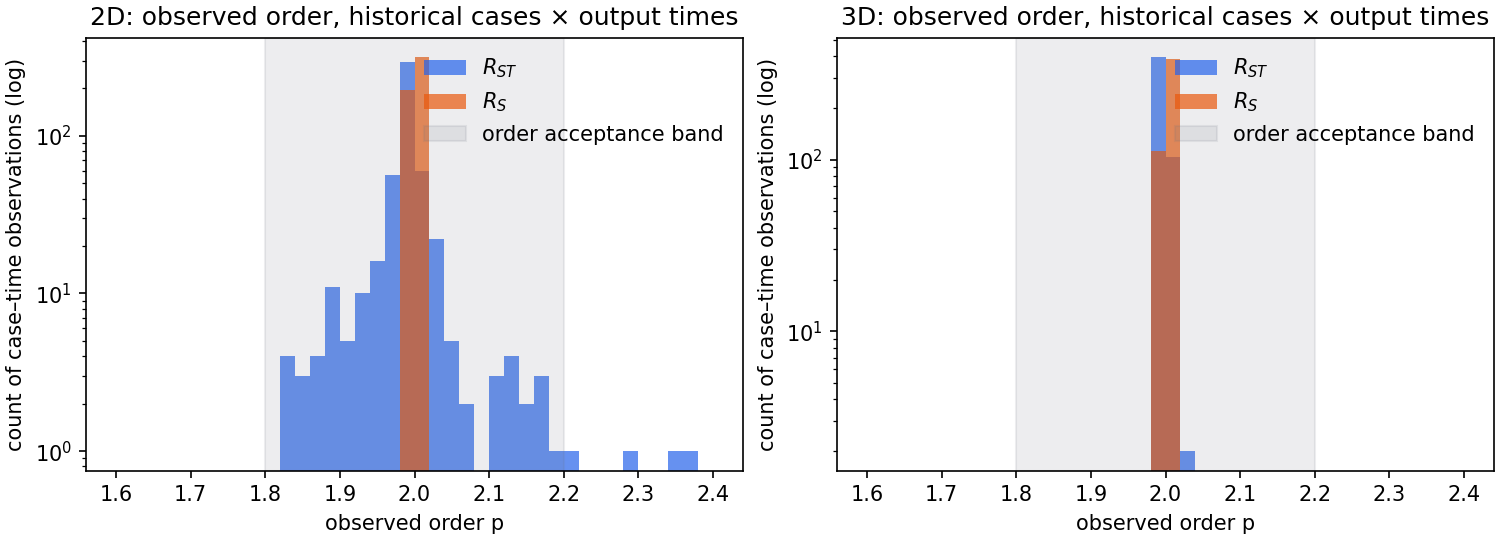
\includegraphics[width=0.48\linewidth]{figs/e0_order.png}\hfill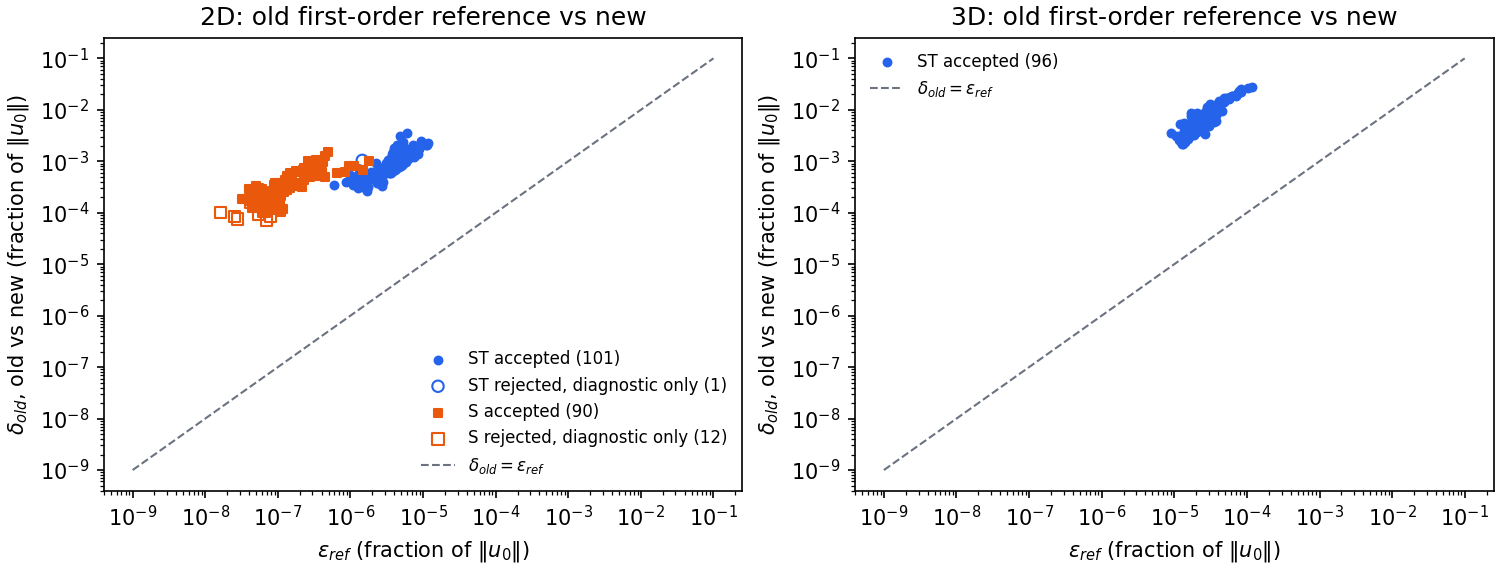
\includegraphics[width=0.48\linewidth]{figs/e0_old_vs_new.png}\end{center}

\subsection*{Caveats and corrections}
\retracted{Amendment A10 replaced the pre-registered cross-check rule (pseudo-spectral order $\ge 2.5$) after the pseudo-spectral data had been seen, though before any comparison with the new references. Under the original rule, only 1/8 2D cross-checks would pass, and 2D would be E0 FAIL. Both verdicts are reported per case. The earlier ``1.7--2.3\,\%'' for the old 3D reference error was too low: the maximum is 2.81\,\%.}
$\epsilon_{ref}$ is a conditional Richardson estimate, not a bound. Sealing is cooperative only: the key sits on the shared cluster account. The sealed cohorts are generated but \textbf{not opened}, and no ROM has been scored on them.

\subsection*{Open}
\begin{itemize}
\item Key custody.
\item Whether to revisit the 2D floor check before opening the sealed cohort.
\item Building the opening tool.
\item A CN-matched space-only reference.
\item Re-scoring every earlier provisional number against this store.
\end{itemize}
